\documentclass[12pt]{beamer}
% \documentclass[10pt]{beamer}

% \usetheme{Pittsburgh}
\usetheme{metropolis}
% \usetheme{Hannover}
% \usetheme{AnnArbor}
% \usetheme{Bergen}
% \usetheme{Berkeley}
% \usetheme{Frankfurt}
% \usetheme{Warsaw}

\usecolortheme{owl} % dark theme
% \usecolortheme[snowy]{owl} % black on white
% \usecolortheme[cautious]{owl}% dark  wo redef colors

\usepackage{appendixnumberbeamer}
\usepackage[T1]{fontenc}
\usepackage[utf8]{inputenc}
% \usepackage{lmodern}
\usepackage{tikz}   

\usepackage{booktabs}
\usepackage[scale=2]{ccicons}

\usepackage{pgfplots}
\usepgfplotslibrary{dateplot}

\usepackage{xspace}
\usepackage{tabularx}

\newcommand{\themename}{\textbf{\textsc{metropolis}}\xspace}

\title{ Hoot AR revenue strategy : HOOT Augmented reality ads}
\subtitle{Performant AR ads with measurable ROI  - making video ads perform using augmented reality}
\date{\today}
\author{Hoot Ar ads team}
\institute{Hoot Live inc., a Delaware C-corp}
% \titlegraphic{\hfill
\includegraphics[height=1.5cm]{logo.pdf}}

\begin{document}

\maketitle

% \begin{frame}{Table of contents}
%   \setbeamertemplate{section in toc}[sections numbered]
%   \tableofcontents[hideallsubsections]
% \end{frame}

% \section{Primer}

\begin{frame}[fragile]{Current landscape in digital video advertising }

\begin{itemize}
\item[-]business model for video advertising is CPM (cost per million impressions) which does not provide accurate ROI for advert buyers
  \pause
\item[-]Many ad-bots end up generating fake views of the video ad creating uncertainty and speculation about the ad’s effectiveness and ROI
\pause
\item[-]Viewers aren’t engaged enough in the ad leading to sales causing major drop off for advertisers
Hoot Network acts as a marketplace, its Open Source software allows anyone to join the network both 
\end{itemize}

\end{frame}
\begin{frame}[t]{Problems of current model}
\begin{itemize}
\item[-]No clear call to actions in video ads
\pause
\item[-]Viewers confused as to what to do after watching video
\pause
\item[-]Unclear ROI to advertisers
\end{itemize}
\pause
Video ads are stuck in the banner ad dark ages pre-Google Adwords 

\end{frame}
\begin{frame}[t]{Hoot Augmented Reality ads }
\begin{itemize}
\item[*]Augmented reality ads create great engagement with users in key ways
\pause
\item[*]Personalization, users can upload photos of themselves and become part of the ad ie their  bitmoji AR avatars (masquerade) 
\pause
\item[*]Content and Virality: celebrities like Rihanna can increase engagement by her presence in an AR ad and can go viral given her popularity
\pause
\item[*]Calls to action: Buy now buttons can be added to the ad, Buy concert ticket to Rihanna event
\end{itemize}
\end{frame}
%--- Next Frame ---%


\begin{frame}[fragile]{Solutions - Building Adwords of video}
\begin{itemize}
\item[+]Clear and engaging call to actions in video ads using AR
\pause
\item[+]Viewers know what to do after watching video by clicking call to action buy 
\pause
\item[+]Clear AR ad performance ROI to advertisers 
\pause
\end{itemize}
Hoot AR ads helps usher a golden age of performant video ads like Google Adwords did to banner ads


\end{frame}
\begin{frame}[t]{CPR model - video Adwords}
\begin{itemize}
\item[*]CPR model using Vickrey auctions allows Hoot to monetize only if the consumer clicks through to advertisers call to action ie charge based on a CPR model cost per referral
\pause
\item[*]This benefits advertisers so they can see clear ROI Referrals > Impressions
\pause
\item[*]This benefits hoot as we can charge based on effectiveness as Google Adwords is able to charge more based on performance laying foundations for a billion dollar ad business
\end{itemize}
\end{frame}
\begin{frame}[standout]
  Hoot AR ads Questions? - building Adwords of the web
  \begin{tikzpicture}
  \node (img1) {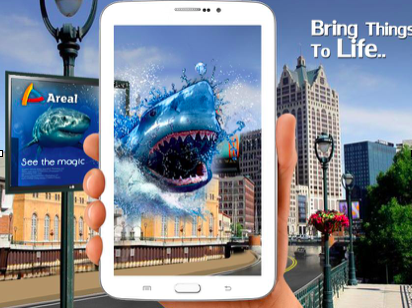
\includegraphics[height=5cm]{static/arad/arad1}};
  % \pause
  \node (img2) at (img1.south east) [xshift=-1cm] {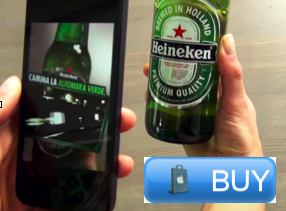
\includegraphics[height=4cm]{static/arad/arad3}};
  % \pause
  \node (img3) at (img2.south west) [xshift=-2cm,yshift=1cm] {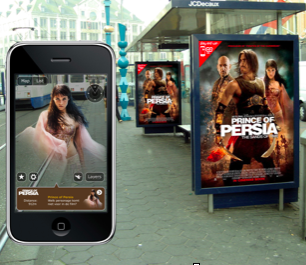
\includegraphics[height=4cm]{static/arad/arad2}};
  \pause
  \node (img4) {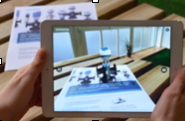
\includegraphics[height=5cm]{static/arad/arad4}};
  % \pause
  \node (img5) at (img1.south east) [yshift=-1cm] {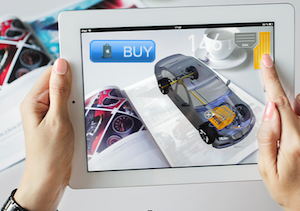
\includegraphics[height=4cm]{static/arad/arad5}};
  
  \end{tikzpicture}
  
\end{frame}

 % \section{Description}

\begin{frame}[allowframebreaks,fragile]{Hoot Augmented Reality ads - Performant AR ads with  measurable ROI - Building Adwords of video}
	
Video Ads have been priced historically based on CPM for impressions as it has been nearly impossible to know how much of these video ads lead to a product sale/conversion or if they even positively affect the customer ROI. Viewers do not know what action to take and how to take the said action leaving them to figure out how to follow up on the video ad they just saw, leading to a lot of drop off and lack of performance of these video ads. Hence It’s not easy  to measure effectiveness and performance of the video ads historically.

Using interactive \textbf{Hoot AR} augmented reality  ads with clear
call to actions such as a buy button or rent button below the
interactive Hoot AR ad, sales can be generated right then and there,
after the viewer interacts with the Hoot AR ad. We will be able to
charge based on sales generated from the AR interaction i.e.,
referrals and instead of pricing based on CPM or impressions we can
price based on  cost per referral(\textbf{CPR}). The CPR price becomes
the signal that drives the continuous auction engine that powers the
Hoot ad marketplace. By bringing about an innovative CPR based
business model to video ads using Augmented reality
\emph{call-to-actions} we bring the effectiveness of Google AdWords to
video ads that only used to perform as well as banner ads
before. Hence Hoot AR ads, improves the effectiveness of plain video
ads, leading to a quantum improvement in video adspend ROI much like
AdWords improved the ROI of web based banner ads, laying the
foundation for a billion dollar ads business.
 	
\end{frame}
 %--- Next Frame ---%


\end{document}
